\section{Result}
This section will present some of the  simulation results.
Simulation settings are:
\begin{itemize}
\item Use 300 historical days to predict future. 
Exclude the weekends and holidays there are around 210
historical pricing days.
\item Use 5 principal components to represent both the curves
and the months. This will capture over 95\% of the variance in data
most of the time.
\item Simulate daily until the end of next month, then do monthly
for another 46 months. Totally there are around 80 forward time points.
\item Simulation was done for contracts of 48 future months.
\item Generate 1000 independent simulations.
\end{itemize}
The simulation can be done in a single PC (P4 2.8G with 2G RAM)
within about 2 hours.

\subsection{Simulation result for a single curve}

Figure \ref{ng-allsim} shows the simulation results 
of NG EXCHANGE for four 2008 futures contracts. 
The fisrt half of the figures plots the historical prices.
The second half is a heat map representation
of all the simulation for daily forward prices, 
where region with darker blue means 
more simulated forward prices fall in there. Five 
randomly chosen forward curves were plotted on top of
the heat map. OU process assumption
guarantees the variances of forward prices become 
constant after some time. 
\begin{figure}[htbp]
\centering
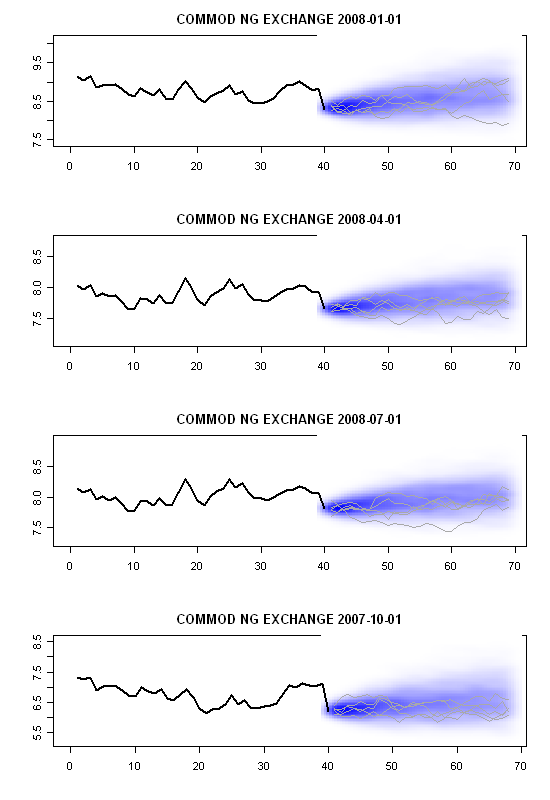
\includegraphics[width=5.5in, height=8in]{figures/ng-exchange-allsim.png}
\caption{Simulation results for NG EXCHANGE: daily forward prices.}
\label{ng-allsim}
\end{figure}

Figure \ref{ng-violin} shows the violin plot for simulated 
monthly forward prices of NG EXCHANGE for four future contracts. 
One can see again the variance
didn't blow up and the simulated forward prices are approximately normal.
\begin{figure}[htbp]
\centering
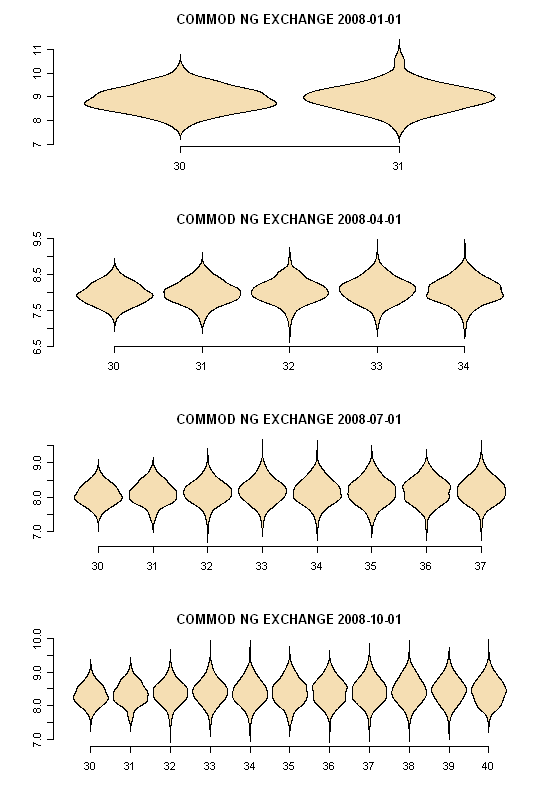
\includegraphics[width=5.5in, height=8in]{figures/ng-exchange-violin.png}
\caption{Simulation results for NG EXCHANGE: violin plot 
for monthly forward prices.}
\label{ng-violin}
\end{figure}

Figure \ref{ng-allmon} shows one simulation for all NG EXCHANGE 
contract months. First panel shows forward prices, the fisrt half is 
for daily and  second half is monthly. We can see the curves 
move almost parallely, so that the correlations among curve 
were preserved. Volatilities in monthly forward
is much highly than daily forward, as it should be. 
Second panel plots the data from another angle, price versus contract 
month. The seasonality was well preserved. Bottom two panels plot the 
same thing for historical data. We can see the similarity 
between forward and historical prices.
\begin{figure}[htbp]
\centering
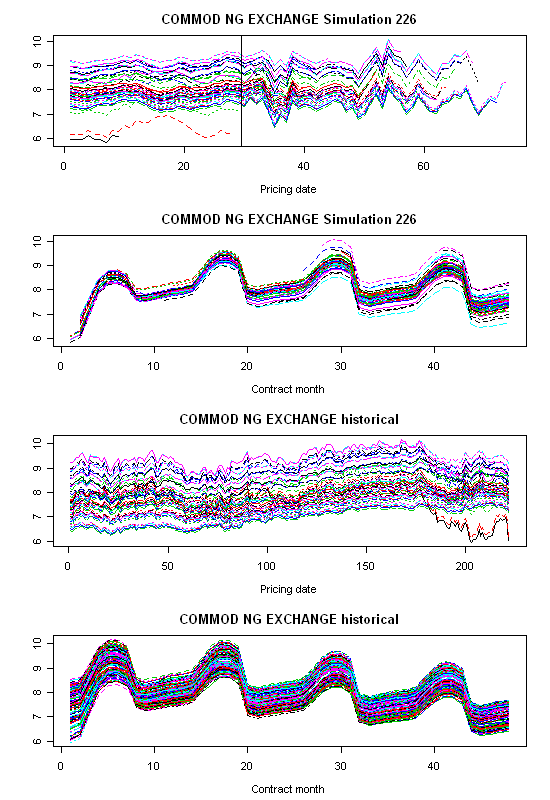
\includegraphics[width=5.5in, height=8in]{figures/ng-exchange-allmon.png}
\caption{One Simulation for NG EXCHANGE all contract months,
versus historical data.}
\label{ng-allmon}
\end{figure}

Table \ref{tbl-ng-vol} summarize the daily, 
weekly and biweekly volatilities of log prices
for simulated NG EXCHANGE prices in log scale, compared with 
historical volatilities. I only showed that for 5 contracts.
One can see the daily and weekly volatilities are faily accurate.
Move to a bigger time horizon, the biweekly volatilities
were underestimated. This result veries by curves 
(some were overestimated) but simulated long term volatilities
are not very accurate in many cases.
This suggests for those curves the OU process assumption 
might be incorrect or unstable(the estimation
of parameters are noisy). 
Some other stochastic process assumptions are worth  trying. 

\begin{table}[htbp]
\begin{center}
\caption{Historical vs. simulated  volatilities for  NG EXCHANGE.}
\begin{tabular}{r|rrrrrr}
\hline
&  2007-10-01 & 2007-11-01 & 2007-12-01 & 2008-01-01 & 2008-02-01\\
  \hline
  \multirow{2}{*}{Daily} & 
  Hist & 0.0228 &  0.0185 &   0.0154 &  0.0144 &  0.0142  \\
 & Sim & 0.0245 &   0.0194 &   0.0154 &  0.0142  & 0.0139 \\ \hline \hline
  \multirow{2}{*}{Weekly} & 
  Hist & 0.0423 &   0.0347 & 0.0291 &  0.0275 &  0.0271 \\
   & Sim & 0.0519 &   0.0390 &   0.0303 &  0.0273 &   0.0267 \\ \hline \hline 
  \multirow{2}{*}{Biweekly} & 
  Hist & 0.0557  & 0.0452 &   0.0378 &   0.0362 &   0.0358 \\
  & Sim & 0.0409 &   0.0356 &   0.0284 &   0.0258 &   0.0254  \\
   \hline
\end{tabular}
\end{center}
\label{tbl-ng-vol}
\end{table}

Figure \ref{heatcontent} shows the simulated vs. historical 
heat content for PWY 5X16 NYC PHYSICAL. One can see the 
distribution of simulated values are consistent with
history.
\begin{figure}[htbp]
\centering
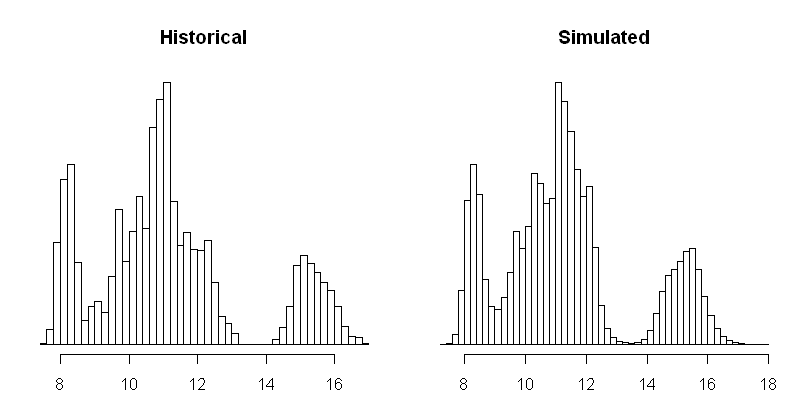
\includegraphics[width=6in, height=3in]{figures/heatcontent-pwy.png}
\caption{Heat content for PWY 5X16 NYC PHYSICAL.}
\label{three-ng}
\end{figure}



\subsection{Multiple curves}
Now we move to view the simulation results for multiple curves.
We want to make sure that the correlations among curves
were preserved in the simulated prices. 

Figure \ref{three-ng} shows one randomly chosen simulation for three 
important NG curves:  NG TENZN6 PHYSICAL,  NG TRAZN6 NY PHYSICAL,
and  NG DOMSP PHYSICAL. These are children curves of NG EXCHANGE
so they were simulated together in the same group. 
We can see historically these
curves are highly correlated. Table \ref{tbl-ng-cor} shows the 
average simulated price correlation vs. historical. The correlations
are a little bit smaller than historical but the error is tolerable.
\begin{figure}[htbp]
\centering
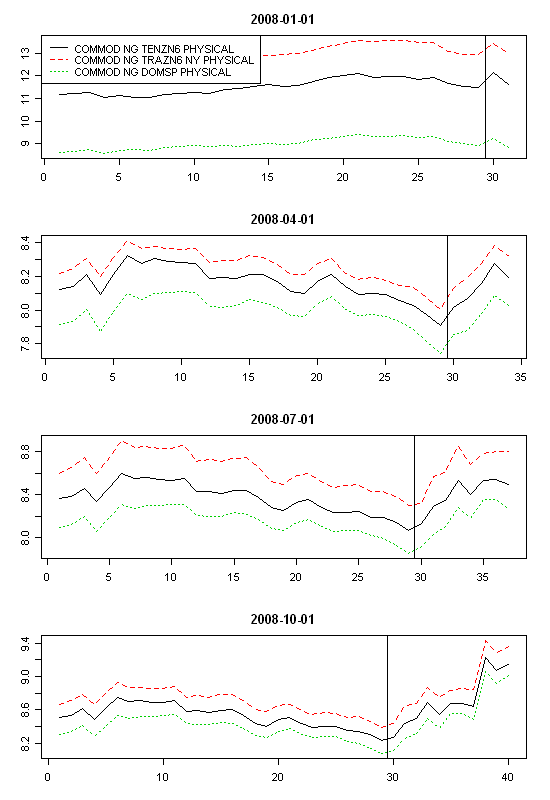
\includegraphics[width=5.5in, height=8in]{figures/ng-multicurve.png}
\caption{One simulation for three Natural Gas curves.} 
\label{three-ng}
\end{figure}

\begin{table}[htbp]
\begin{center}
\caption{Historical vs. simulated correlations among three NG curves.}
\begin{tabular}{rrrr|rrr}
  \hline
 &  \multicolumn{3}{c|}{Historical} &  \multicolumn{3}{|c}{Simulated} \\ \hline
 & TENZN6  & TRAZN6 NY  & DOMSP  & TENZN6  & TRAZN6 NY  & DOMSP  \\
  \hline
TENZN6  & 1.0000 & 0.9988 & 0.9983 & 1.0000 & 0.9737 & 0.9640 \\
  TRAZN6 NY  & 0.9988 & 1.0000 & 0.9976 & 0.9737 & 1.0000 & 0.9763 \\
  DOMSP  & 0.9983 & 0.9976 & 1.0000 & 0.9640 & 0.9763 & 1.0000 \\
   \hline
\end{tabular}
\end{center}
\label{tbl-ng-cor}
\end{table}

Now we move to children curves in different groups.
We picked three electricity curves
PWX 5X16 BOS PHYSICAL, PWJ 5X16 BGE PHYSICAL
and PWY 5X16 NYC PHYSICAL.
Those curves belong to different markets
so correlation among them are passed on from their parents.
Figure \ref{three-elec} plots result from one simulation.
The prices was shifted and scaled 
so that they have the same mean and standard deviation.
\begin{figure}[htbp]
\centering
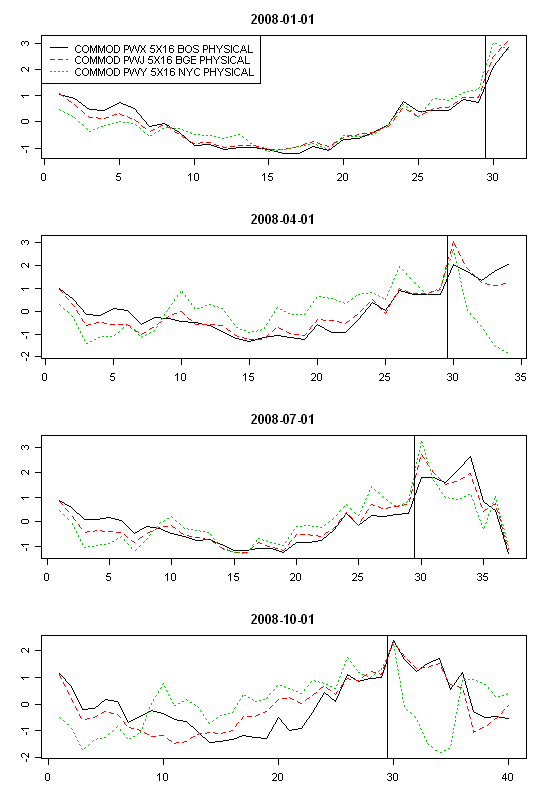
\includegraphics[width=5.5in, height=8in]{figures/elec-multicurve.png}
\caption{Simulation for three electricy curves.} 
\label{three-elec}
\end{figure}

Table \ref{tbl-elec-cor} summarizes the correlation among them.
This time the correlations in simulation were obviously
underestimated, dropped to around 0.8 from 0.9.

\begin{table}[htbp]
\begin{center}
\caption{Historical vs. simulated correlations among three electricity curves.}
\begin{tabular}{rrrr|rrr}
\hline
 &  \multicolumn{3}{c|}{Historical} &  \multicolumn{3}{|c}{Simulated} \\ \hline
 &  5X16 BOS  &  5X16 BGE  &  5X16 NYC  &  5X16 BOS  &  5X16 BGE  &  5X16 NYC  \\
  \hline
 5X16 BOS  & 1.0000 & 0.8673 & 0.9317 & 1.0000 & 0.8052 & 0.8205 \\
   5X16 BGE  & 0.8673 & 1.0000 & 0.9414 & 0.8052 & 1.0000 & 0.8813 \\
   5X16 NYC  & 0.9317 & 0.9414 & 1.0000 & 0.8205 & 0.8813 & 1.0000 \\
   \hline
\end{tabular}
\end{center}
\label{tbl-elec-cor}
\end{table}

A little  calculation can show why we got this result.
Let $X$, $Y$ and $Z$
be random variables. $cor(X,Y)=\rho_1$, $cor(Y,Z)=\rho_2$. 
Let the correlation between $X$ and $Z$ be $\rho$. 
When $\rho_1$ and $rho_2$ are faily large (bigger than
$\sqrt(2)/2$, to be exact), $\rho$ can be as low as 
$cos(cos^{-1}(\rho_1)+cos^{-1}(\rho_2))$. When $\rho_1=\rho_2=0.99$, 
we have $\rho \ge 0.96$, which can be seen from Table 
\ref{tbl-ng-cor}. For $\rho_1=\rho_2=0.9$, $\rho \ge 0.62$.
We can see when $\rho_1$ and $rho_2$ dropped a little bit,
$\rho$ dropped quickly. 
So when the correlations between children and parents are
not VERY high (0.9 is high correlation but not high enough),
correlations in simulated children could drop very quickly. 
One solution for this problem is to further cut the regions into
smaller subregion, and assign more parent curves to the children.
That way the children can correlate each other through 
many different paths and the result will be more reliable.
